\documentclass{llncs}
\usepackage{graphicx,psfig,amsmath,float,epstopdf,multirow,mathtools,changepage,amssymb}
\usepackage[para,online,flushleft]{threeparttable}
\usepackage{float} % lets you have non-floating floats
\usepackage{url} % for typesetting urls
\usepackage{caption}
\usepackage{program}
\usepackage{tabularx}
\usepackage{colortbl}
\usepackage{algorithm, algpseudocode}

%\usepackage{mathtools}
\usepackage{etoolbox}
\usepackage{hhline}
\usepackage{subcaption}
\newfloat{fig}{thp}{lof}[section]
\floatname{fig}{Figure}
\let\bbordermatrix\bordermatrix
\patchcmd{\bbordermatrix}{8.75}{4.75}{}{}
\patchcmd{\bbordermatrix}{\left(}{\left[}{}{}
\patchcmd{\bbordermatrix}{\right)}{\right]}{}{}


\title{
Optimization of Location Allocation of Web Services using non-dominated sorting algorithm(NSGA-II)
}

\author{Boxiong Tan, Hui Ma, Mengjie Zhang}
\institute{School of Engineering and Computer Science,
\\Victoria University of Wellington, New Zealand \\
\email{\{Boxiong.Tan, Hui.Ma, Mengjie.Zhang\}@ecs.vuw.ac.nz}}

\makeatletter
\usepackage[pdfauthor={\@author}, pdftitle={\@title}]{hyperref}
\makeatother

\begin{document}

\maketitle

\begin{abstract}
In recent years, web services technology is becoming increasingly popular because the convenience, 
low cost and capacity to be composed into high-level business processes. 
The service location-allocation problem for a web service provider is critical and urgent. 
It is because some factors such as Network latency, can make serious effect on the quality of service (QoS). 
This paper presents a multiobjective optimization algorithm based on NSGA-II to solve the service location-allocation problem. 
A stimulated experiment is conducted using the WS-DREAM dataset. 
The results were compared with a single objective algorithm: Integer programming and greedy optimization (IPGO). 
It shows NSGA-II based algorithm can provide a set of best solutions that outperforms IPGO.
\end{abstract}

\section{Introduction}
Web Services are considered as self-contained, self-describing, modular applications that can be published, located, and invoked across the Web \cite{Ran}. 
In recent years, web services technology is becoming increasingly popular because the convenience, low cost and capacity to be composed into high-level business processes \cite{Aboolian}.
Because of modularization and open interfaces, Web services facilitate the development of highly 
customizable and adaptable applications to meet business demands. Furthermore, Web services offer a 
convenient registration, search  and discovery system.

With the ever increasing number of functional similar web services being available on the Internet, the web service providers (WSPs) are trying to improve the quality of service (QoS) to become competitive in the market.  
QoS also known as non-functional requirements to  web services, is the degree to which a service meets specified requirements or user needs \cite{4061431}, such as response time, security and availability. 
Among numerous QoS measurements, service response time is a critical factor for many real-time services, e.g. traffic service or finance service. 
Service response time has two components: transmission time (variable with message size) and network latency \cite{Johansson}. 
Study \cite{916684} shows that network latency is a significant component of service response delay.
Ignoring network latency will underestimate response time by more than 80 percent. Since network latency is related to network topology as well as physical distance \cite{distanceMetrics}. 
The network latency could also vary with the network topology changes.
The only way to reduce the network latency is to move the service to a location where has lower network latency to the user center. 
Hence, the WSPs need to consider which physical locations to deploy their services so that it could minimize the cost as well as ensure the QoS.

The Web service location-allocation problem is essentially a multi-objective optimization problem \cite{Multiobjective}, for which there are two conflict objectives, to provide optimal 
QoS to service users and to consume minimal deployment cost.
Ideally, WSP could deploy their services to each user center in order to provide the best quality.
However, the more services deployed, the better the quality and the higher cost. 
This problem is considered as NP-hard due to the fact that the combinatorial explosion of the search space \cite{Vanrompay}. 


Very few researches study this problem, most of the researchers treat this problem as a single objective problem.
\cite{Aboolian} \cite{Sun} try to solve the problem by using integer linear programming techniques.
In particular, \cite{Sun} solved this problem by employing a modified Alternate Location-Allocation (ALA) and greedy algorithm. 
However, essentially Sun's approach build upon integer programming and greedy optimization. 
As a result, the solution is easily stuck at local optima.
Huang \cite{EnhancedGenetic} propose an enhanced genetic algorithm (GA)-based approach which make use of the integer scalarization technique to solve this problem.
GA \cite{man1996genetic} is an Evolutionary algorithm (EA) that uses genetic operators to obtain optimal solutions without any assumptions about the search space.
This algorithm solves the problem with one objective and one constraint, however there are a few disadvantages existed in
integer scalarization technique \cite{Multiobjective}, which were discussed explicitly in Section \ref{sec:Background}.

Since the location-allocation should be considered as a multi-objective problem. Evolutionary multi-objective optimization (EMO) methodologies have to be considered.
Evolutionary multi-objective optimization (EMO) methodologies are a subset of Evolutionary algorithms (EA), which have been used in solving multi-objective optimization problems in recent years. 
EMO are ideal for solving multi-objective optimization problems \cite{key:article}, since EMO works with a population of solutions, 
a simple EMO can be extended to maintain a diverse set of solutions.
With an emphasis for moving toward the true Pareto-optimal region, an EMO can be used to find multiple Pareto-optimal solutions in 
one single simulation run \cite{OptimizationElectrical}. Among numerous EMO algorithms,
Non-dominated sorting GA (NSGA-II) \cite{996017}, Strength Pareto Evolutionary Algorithm 2 (SPEA-2) \cite{Deb} have become standard approaches. 
Some schemes based on particle swarm optimization approaches \cite{Elhossini} \cite{Huang} are also important. 
NSGA-II is one of the most widely used methods for generating the Pareto frontier. 
NSGA-II implements elitism and uses a phenotype crowd comparison operator that keeps diversity without specifying any additional parameters \cite{Deb06referencepoint}.
In this paper, we propose to use NSGA-II to solve the web service location-allocation problem.

To show the effective and efficiency of our proposed NSGA-II based approach, we conduct an experiment to compare our approach with
traditional approach based on integer programming and greedy optimization (IPSO). IPSO models one objective as an assignment problem then uses integer programming techniques to 
obtain an optimal solution. Then, based on this solution, the algorithm further optimize the other objective using greedy algorithm. 
The major advantage of IPSO is that it is very efficient and gives 
an reasonably good result. On the other hand, the objectives are considered unevenly. That is, IPSO considers the objective which optimize by linear programming as its priority.


The aim of this research is to provide a framework that guides a WSP to locate services.
We consider the problem faced by a WSP who has existing facilities but wishes to use the collected data to re-allocate their services in order to maximum their profit.
The WSP must decide on facility locations from a finite set of possible locations. 
In order to make the decision, the WSP must first analyze the data collected from current use of services. 
The collected data should includes the records of invocations from each unique IP address.
Therefore, based on these data, the WSP could summarize several customer demands concentrated at \textit{n} discrete nodes \cite{Aboolian}, namely user centers. 
We assume the WSP has already done this step and list of user centers and candidate service deployment locations are given.
In addition to decide which location to re-allocate the services, a dataset which contains the network latency between demand a user center and a candidate location are critical. 
The WSP could collect the data or use existed dataset  \cite{6076756} \cite{5552800}. 
Then, the service provider could use the algorithm which proposed by this paper, to select an optimal plan based on their funds. 
The algorithm will produce a near optimal solution which indicate the services deployment locations with a minimum cost and best service quality.
The main objectives are:
\begin{itemize}
	\item To model the web service location-allocation problem so that it can be tackled with NSGA-II
	\item To develop a modified NSGA-II approach for the web service location-allocation problem
	\item To evaluate our approach by comparing it to a linear assignment with greedy optimization (IPGO) algorithm.
\end{itemize}

In Section \ref{sec:Background} we introduce the background of NSGA-II and IPGO as well as discuss the work from previous researchers.
In Section \ref{sec:problem} we provide a formulation for our model. Section \ref{sec:algorithm_des} develops a modified NSGA-II. 
We use these to study a number of hypotheses on the placement of WSPs. These solutions are compared to solutions from Integer
programming with greedy optimization(IPGO). 
The experimental design was discussed in Section \ref{sec:experiment}. The experimental results are shown in Section \ref{sec:results}.


\section{Related Works and Background}
\label{sec:Background}
A few researchers attempt to solve the service location-allocation problem by using single objective approach. Most of them solve this problem with linear programming approaches.
\cite{5961695} considers more than 3 objectives: response time, availability and cost. 
It solves the placement of Datacenters for Internet Services with simulated annealing plus linear programming. 
Sun et.al proposed two approaches \cite{Aboolian} \cite{Sun} that employ LP and DAL respectively. 
The first approach \cite{Aboolian} assumes the model is based on a duopoly competitive market.
The second approach \cite{Sun} assumes multiple competition services have been established in the market.
Some researchers use evolutionary algorithms. Huang \cite{EnhancedGenetic} applied an enhanced GA algorithm which employ the integer scalarization technique \cite{Multiobjective}. However, 
the integer scalarization technique has many disadvantages:
\begin{enumerate}
	\item The decision maker needs to choose an appropriate weights for the objectives to retrieve a satisfactorily solution.
	\item The algorithm does not produce an uniform spread of points on the Pareto curve. That is, all points are grouped in certain parts of the Pareto front.
	\item Non-convex parts of the Pareto set cannot be reached by minimizing convex combinations of the object functions.
\end{enumerate}

So far, there is no research consider the service location-allocation problem as a multi-objective problem. Therefore, this paper is the first attempt to solve this problem using 
multi-objective algorithm.

\subsection{NSGA-II}
NSGA-II \cite{996017} belongs to the larger class of genetic algorithm (GA). GA \cite{man1996genetic} is a powerful tool to solve combinatorial optimization problems. It is an iterative procedure based on a constant-size population. In a GA, a population of strings (called chromosomes
or the genotype of the genome), which are encoded as candidate solutions (called individuals, creatures, or phenotypes) to an optimization problem, evolves towards better solutions. 
Each genome is associated with a fitness value based on a fitness function that indicates how close it comes to meeting the overall specification, when compared to other genomes in the
population. The fitness value of an individual is also an indication of its chances of survival and reproduction in the next generation. A typical genetic algorithm requires a genetic
representation of the solution domain and a fitness function to evaluate the solution domain. Since a chromosome from the population represents a solution, when the algorithm starts, 
the whole population moves like one group towards an optimal area, so the GA searches from a population of solutions rather than a single solution.

NSGA-II is a multi-objective algorithm based on GA. When used for problems with only two objectives, NSGA-II performs 
relatively well in both convergence and  computing speed. It permits a remarkable level of flexibility with regard to 
performance assessment and design specification. NSGA-II assumes that every chromosome in the population has two 
attributes: 1) a non-domination rank in the population, 2) a local crowding distance in the population. The goal of 
NSGA-II is to converge to the Pareto front as possible and with even spread of the solutions on the front by 
controlling the two attributes. 

The algorithm starts with initialization population. Once the population is sorted based on non-domination sorting, rank is assigning to each chromosome.
Then, a parameter called crowding distance is calculated for each individual. The crowding distance is a measure of how close an individual is to its neighbors. Large 
average crowding distance will result in better diversity in the population. 

Parents are selected from the population by using tournament selection based on the rank and crowding distance. An individual is selected in the rank is lesser than the other or 
if crowding distance is greater than the other. The selected population generates offsprings from crossover and mutation operators. 

The population with the current population and current offsprings is sorted again based on non-domination and only the best N individuals are selected, where N is the population size.
The selection is based on rank and the on crowding distance on the last front.

\subsection{Integer programming with Greedy Optimaization (IPGO)}

Linear assignment \cite{lawler1963quadratic} is a special case of the transpotation problem, which is a special case of the minimum cost flow problem, which
in turn is a special case of a linear program.

Much research has been devoted to develop efficient heuristic algorithm to solve location-allocation problem. Two of the predominant
greedy construction heuristics are the ADD and DROP \cite{Sun} methods, which build solutions from scratch. 
The ADD procedure starts with all facilities closed and locates a facility that gives the greatest savings at each step and 
iterates through all potential locations until no further savings can be made. In contrast, DROP opens all facilities and removes a 
location that gives the greatest savings at each step and tries to find optimal or near optimum solutions at the end of the 
iterative procedure. Integer programming with greedy optimization(IPGO) builds upon ADD and DROP methods. 
In order to solve multi-objective problem, IPGO first employ Integer programming to derive a minimum cost solution. Then, it
uses a greedy procedure to optimize the other objective.

Sun et.al proposed Drop, ALA, and LP relaxations of Integer transpotation problem (DAL) \cite{Sun} is very similar with this approach. 
The DAL heuristics provided near optimal solutions in short computer times and with limited computer memory. But in Sun's approach, 
he assumes there is competitive service providers existed. In contrast, IPGO does not consider about existed services. Therefore, IPGO
uses Linear assignment approach instead of Alternate Location-allocation (ALA).



\section{Problem Description and Modeling}
\label{sec:problem}
In this section, we first describe the service location-allocation problem in details, then we will present models for the services location allocation problem.

\subsection{Problem Description}
Web service location-allocation problem is to determine reasonable locations for web services so that deployment cost of WSP can be minimized while service performance can be optimized.
In this paper, to optimize service performance we consider to minimize network latency.

The task of service location allocation has two objectives:
\begin{itemize}
	\item To minimize the total cost of the services.
	\item To minimize the total network latency of the services.
\end{itemize}


\subsection{Model Formulation}
To model service location-allocation problem we need to make use of a set of matrices, to present input information and output solutions. 

For service location-allocation problem we needs information of service usage, network latency, and service deployment cost to decide service location-allocation so that the overall network latency can be minimized with minimal deployment cost and with constraint.
Assume a set of $S = \{ s_{1}, s_{2}, ..., s_{x}\}$ services are
requested from a set of location $I = \{ i_{1}, i_{2}, ..., i_{y} \}$. The service providers allocate services 
to $J = \{ j_{1}, j_{2}, ..., j_{z} \}$ be the set of candidate facility locations.
To model the service location-allocation problem we use five matrices: 
service network latency matrix $L$, service location
matrix $A$, service invocation frequency matrix $F$, cost matrix $C$ and user response time matrix $R$.

In the following we list a set of notations that will be used for modelling. 
{
\centering
	\begin{tabular}{l*{2}{l}r}
		\hline
		\textbf{Sets} \cr
		$S$	& set of service $S = \{s_{1}, s_{2}, ..., s_{s}, s_{x}\}$ \cr
		$I$	& set of user center $I = \{i_{1}, i_{2}, ..., i_{i}, i_{y}\}$ \cr
		$J$	& set of candidate location $J = \{j_{1}, j_{2}, ..., j_{j}, j_{z}\}$ \cr
		\textbf{Matrices} \cr
		$L$ & server network latency matrix $L = \{l_{ij}\}$ \cr
		$A$ & service location matrix $A = \{a_{sj}\}$ \cr
		$F$ & service invocation frequency matrix $F = \{f_{is}\}$ \cr
		$C$ & cost matrix $C = \{c_{sj}\}$ \cr
		\hline
	\end{tabular}
\\
}
The service invocation frequency matrix $F= [f_{is}]$, is used to record services invocation frequency from user centers, 
which $f_{is}$ is an integer that indicate the number of invocation in a period of time from user center to service. 
For example, $f_{13}$ = 85 denotes service $s_{1}$ is invocated 85 times in a predefined period of time.

\parbox{.45\linewidth}{
{\centering
$
F = \bbordermatrix{~ & s_{1} & s_{2} & s_{3}  \cr
					i_{1}	&120 &35 &56	\cr
					i_{2}	&14  &67 &24 \cr
					i_{3}	&85 &25 &74 \cr}
$
\\}
}
\parbox{.45\linewidth}{
{\centering
$
L = \bbordermatrix{~ & j_{1} & j_{2} & j_{3} \cr
					i_{1}	&0 &5.776 &6.984	\cr
					i_{2}	&5.776  &0 &2.035 \cr
					i_{3}	&0.984 &1.135	&2.3 \cr}
$
\\}
}

The network latency matrix $L = [l_{ij}]$, is used to record network latency from user centers to 
candidate locations. For example, The network latency between user center $i_{2}$ with candidate location $j_{1}$ 
is 5.776s. These data could be collected by monitoring network latency \cite{6076756} \cite{5552800}.

The cost matrix $C = [c_{sj}]$, is used to record the cost of deployment of services from candidate locations, 
which $c_{sj}$ is an integer that indicate the cost of the deploying services from a candidate location. 
For example, $c_{12} = $ 80 denotes the cost of deploying service $s_{1}$ to location $j_{2}$ is 80 units.

\parbox{.45\linewidth}{
{\centering
$
C = \bbordermatrix{~ & j_{1} & j_{2} & j_{3}\cr
					s_{1}	&130 &80 &60\cr
					s_{2}	&96  &52 &86\cr
					s_{3}	&37 &25 &54\cr}
$
\\}
}
\parbox{.45\linewidth}{
{\centering
$
A = \bbordermatrix{~ & j_{1} & j_{2} & j_{3}\cr
					s_{1}	&0 &1 &0	\cr
					s_{2}	&0  &0 &1	\cr
					s_{3}	&1 &1 &0	\cr}
$
\\}
}

To model the service location-allocation problem we Consider the following assumptions:
\begin{enumerate}
	\item The new WSP decides where to locate his facilities regardless if there is existed functional similar services from other WSPs.
	\item The decision of service location-allocation is made only considering two factors: total network latency and total cost.
	\item A static allocation policy is used by WSPs. In practice, Web Services typically offer clients persistent and interactive services, which often span over multiple sessions. Therefore, a dynamic reallocation scheme is not practical as it may disrupt the continuity of the services.
\end{enumerate}


The service location-allocation matrix $A = [a_{sj}]$ represents the actual service location-allocation, where $a_{sj}$  is a binary value i.e. 1 or 0.


Using service location allocation matrix $A = [a_{sj}]$ and network latency matrix $L = [l_{ij}]$, we can compute user
response time matrix $R = [r_{is}]$. 

{\centering
	\begin{equation}
		r_{is} = MIN\{l_{ij} \mid j \in \{1, 2, ..., z\} \text{ and } a_{sj} = 1\}
	\end{equation}
\\}
For example, we use two matrices $L$ and $A$ mentioned above to construct response time matrix $R$. 
For each services $s$, by checking matrix $A$, find out which location the service has been deployed.
Then look back matrix $L$, find out its corresponding latency to each user center $i$. If there is
more than one location, then the smallest latency is selected. Therefore, we can construct the response time matrix $R$ as:

{\centering
$
R = \bbordermatrix{~ & s_{1} & s_{2} & s_{3}\cr
					i_{1}	&5.776 &6.984 &0	\cr
					i_{2}	&0  &2.035 &0	\cr
					i_{3}	&1.135 &2.3 &0.984	\cr}
$
\\}


\section{NSGA-II For Web Services Location Allocation}
\label{sec:algorithm_des}
To apply NSGA-II to the service location-allocation problem, the first step is to define the variable in NSGA-II, i.e. to
identify chromosome, genetic operators and the fitness functions.

\subsection{Chromosome Representation and Constraints}
We use the service location matrix $A$ = $[a_{sj}]$ as the representation of chromosome that we mentioned in Section 
\ref{sec:problem}.

The constraint setting is based on service providers' needs. One can set multiply constraints to the problem to narrow the potential searching space.
In our case, we set two basic constraints: The first constraint guarantees that each service is deployed in at 
least one location.

{\centering
	\begin{equation}
		\sum\limits_{x \in S} a_{xj} \geq 1
	\end{equation}
\\}

The second constraint is the cost constraint which predefined the upper boundary of the total cost.
An integer number $CostLimitation$ is defined.

{\centering
	\begin{equation}
		\sum\limits_{s \in S} \sum\limits_{j \in J} c_{sj} \times a_{sj} \leq CostLimitation
	\end{equation}
\\}


\subsection{Genetic Operators}
\label{sec:operators}
 The original NSGA-II uses a simulated 
binary crossover (SBX) \cite{930314} and polynomial mutation \cite{Raghuwanshi04} to cope with continuous problem. 
However, our problem is discretized, therefore we use the regular GA mutation and crossover operations.

The selection operator is the tournament selection \cite{Xie:2008:AMI:1389095.1389347}, which allows the highest probability 
of being reproduced to next generation.

\subsubsection{Mutation}
The mutation operator works as follows: Initially choose one random location from the chromosome. 
Then, reverse the bit, e.g. 0 to 1 or 1 to 0. 

In this study, a chromosome in a population will be selected based on mutation possibility $P_{m}$. $P_{m}$ is 
a parameter predefined and fixed.
As shown in below, a random position will be selected and replaced by a reversed number.
%\begin{figure}[ht]
%\centering
	%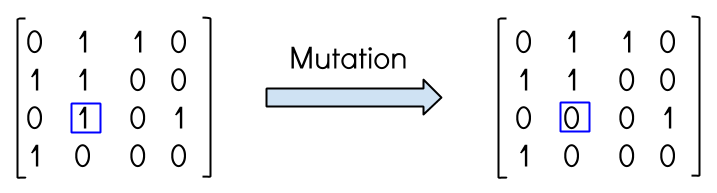
\includegraphics[width=0.5\textwidth]{pics/mutation.png}
%\caption{}
%\label{graph1}
%\end{figure}
\subsubsection{Crossover}
The crossover operator in this paper is the single point crossover. 
The crossover is controlled by crossover probability $P_{c}$. $P_{c}$ is a parameter predefined and fixed.
The crossover point is created randomly within the length of the chromosome. 
As in the example below, two parents crossover at a point, to generate two offsprings.
%\begin{figure}[ht]
%\centering
	%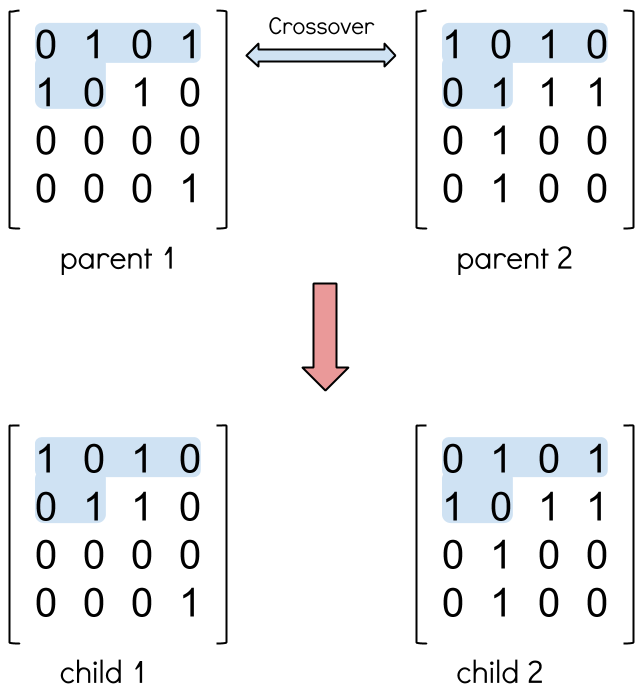
\includegraphics[width=0.5\textwidth]{pics/crossover.png}
%\caption{}
%\label{graph2}
%\end{figure}

\subsubsection{Fitness Function}

\begin{flushleft}In order to accomplish these two objectives. We design two fitness functions to evaluate 
how good each chromosome meets the objectives.\end{flushleft}
\subsubsection{Cost fitness function}

\begin{equation}
		CostFitness = \sum\limits_{s \in S} \sum\limits_{j \in J} c_{sj} \times a_{sj}
\end{equation}

$c_{sj}$ is the Cost matrix stores the cost information of service $s$ at location $j$. $a_{sj}$ represents the deployment plan. The sum of the multiplication of 
$c_{sj}$ and $a_{sj}$ derives the total cost of the deployment plan.


\begin{flushleft}For example, we use the above mentioned matrices $C$ and $A$.\end{flushleft}

%\begin{align*}
	$
	CostFitness &= c_{11} * a_{11} + c_{12} * a_{12} + c_{13} * a_{13} + ... + c_{33} * a_{33} \\
	&= 130 * 0 + 80 * 1 + 60 * 0 + ... + 54 * 0 \\
	&= 228
	$
%\end{align*}
\subsubsection{Network latency fitness function}

We assume the latency is symmetrical between user center and candidate location. e.g. 
The latency from location $i$ to location $j$ is same with the latency from location $j$ to location $i$.

	\begin{equation}
		LatencyFitness = \sum\limits_{i \in I} \sum\limits_{s \in S} r_{is} \times f_{is}
	\end{equation}

\begin{flushleft}For example, we use the above mentioned matrices F and R.\end{flushleft}

%\begin{align*}
	$
	LatencyFitness &= f_{11} * r_{11} + f_{12} * r_{12} + f_{13} * r_{13} + ... + f_{33} * r_{33} \\
	&= 120 * 5.776 + 6.984 * 35 + 0 * 56 + ... + 0.984 * 74\\
	&= 1300.696
	$
%\end{align*}



\subsection{NSGA-II based algorithm for service location-allocation}
Algorithm \ref{NSGA2} shows the precedure of NSGA-II applied on service location-allocation problem.
\begin{algorithm}[htb]
	\caption{NSGA-II for service location-allocation}
	\label{NSGA2}
	\textbf{Inputs:}
		Cost Matrix $C$,
		Server network latency matrix $L$, 
		Service location matrix $A$, 
		Service invocation frequency matrix $F$

	\textbf{Outputs:}
		Pareto Front: A set of Service allocation matrix $A$

	\begin{algorithmic}[1]
		\State Initialize a population of chromosome with random binary value
		\State Evaluate population with fitness functions
		\State Non-dominated sort and assign ranking to each chromosome
		\State Evaluate the Crowding distance of each chromosome
		\State Initialize the Pareto Front Pool
		\While{predefined generation}
		\State Apply Tournament Selection
		\State Apply Crossover 
		\State Apply Mutation
		\For( each chromosome)
		\While{ violate service number constraint}
		\State Deploy the service to a random candidate location
		\EndWhile
		\While { violate cost constraint}
		\State Shut down a service from a random location as long as it does not violate service number constraint
		\If { no service can be closed}
		\State Break
		\EndIf
		\EndWhile
		\If{ chromosome does not exist in the Pareto front Pool}
		\State Evaluate with fitness functions
		\EndIf
		\State Non-dominated sort and assign ranking
		\State Evaluate the Crowding distance
		\EndFor
		\State Recombination and Selection
		\State Update Pareto Front Pool with current Pareto Front
		\EndWhile
		\State Return Pareto Front
	\end{algorithmic}
\end{algorithm}

There are two major differences between standard NSGA-II and modified version. Firstly, in order to avoid repeat evaluation of the fitness
of chromosome which contribute to the majority of computation. After the first generation is initialized, the Pareto front will be 
stored in the memory. In each generation, when evaluate the chromosome, the chromosome will be checked whether it is existed in the memory pool. 
If so, then the calculation of fitness will be skipped. At the end of each iteration, the Pareto front pool will be updated to the current Pareto front.
The reason for setting a memory pool is that, after a number of iterations, the population start converging. 
Most of the population are redundant. Therefore, a memory pool could considerably reduce the repeat computation.

The other difference is that, we use general mutation and crossover operation instead of polynomial mutation and simulated binary crossover.
It is important to note that mutation and crossover operators can produce solutions that might violate the constraints. 
Therefore, repair operators are needed to try to maintain feasible solutions. The repair operators are essentially while 
loop which repeatedly check if the chromosome violates constraints.

Worth noting that the cost constraint repair operator may not provide a strictly correct solution that satisfied the cost constraint.

\section{IPGO for Web Service Location Allocation}
\begin{algorithm}[htb]
	\textbf{Inputs:}
		Cost Matrix $C$,
		Server network latency matrix $L$, 
		Service location matrix $A$, 
		Service invocation frequency matrix $F$

	\textbf{Outputs:}
		Service location matrix $A$
	\caption{IPGO for service location-allocation}
	\label{IPGO}
	\begin{algorithmic}[1]
		\State initialize allocation matrix $A$ = \{1\}.
		\State Optimize cost solution $A$ with Integer assignment solver.
		\State Evaluate Cost fitness with Cost fitness function
		\For( each row of A)
			\For( each column of A)
				\If {$A_{ij}$ = 0}
					\State Start the service: $A_{ij}$ = 1
					\State Evaluate $A$ with Network Latency fitness function.
					\If {Current Network latency fitness is greater than previous fitness}
						\State Change back $A_{ij}$ = 0
					\EndIf
				\EndIf
			\EndFor
		\EndFor
		\State Return Service location matrix $A$
	\end{algorithmic}
\end{algorithm}
In order to solve the location allocation problem with IPGO. We model the cost objective as the priority, optimize with Linear programming.
The cost matrix $C$ and solution matrix $A$ are identical with the two matrices defined in Section \ref{sec:problem}. We use the same fitness functions as in NSGA-II to 
evaluate the Cost objective and Latency objective.

%\begin{equation}
     %\begin{align}
       %\mbox{Minimize } & \sum\limits_{s \in S} \sum\limits_{j \in J} c_{sj} \times a_{sj} \\
       %\mbox{Subject to} & \\
			%& \sum\limits_{s} A_{sj} = 1 (s = 1, 2, ...),\\
	        %& \sum\limits_{s \in S} \sum\limits_{j \in J} C_{sj} \times A_{sj} \leq CostLimitation \\
		%\mbox{and } & A_{sj} = $0 or 1$ (s, j = 1, 2, ...) \\
     %\end{align}
%\end{equation}

Once a minimum cost solution is found by linear assignment, the solution set will be passed to the ADD procedure to serve as an initial solution for 
further improvement on Network latency.

 The ADD procedure as follows:
\begin{itemize}
	\item Evaluate network latency fitness of the initial solution.
	\item Starts a facility then evaluate with network latency fitness function. If the network latency fitness decreased as well as 
		the cost fitness does not exceed the cost constraint. The solution is kept.
	\item If there is no location could be choose, terminate the procedure.
\end{itemize}




\section{Experiment Design}
\label{sec:experiment}
The purpose of the experiment is comparison between Integer programming and greedy optimization (IPGO) with NSGA-II in terms of efficiency and quality of solutions. 

The exact algorithm was coded in R \cite{Morandat:2012:EDR:2367163.2367172} using packages: NSGA2R and LpSolve. The program was run on a 3.40GHz 
desktop computer with 8 GB RAM.

To compare with IPGO, four different datasets were used, the problem instance was generated as follows:
\begin{enumerate}
	\item The potential user center and candidate locations were randomly selected from existed network latency dataset \cite{6076756} \cite{5552800}. 
	\item The number of potential user center equals the candidate locations. We defined 4 different size of allocation matrices:
			$3 \times 3, 5 \times 5, 10 \times 10$ and $15 \times 15$.
		\item Network latency $L_{ij}$ were selected from public WS-DREAM dataset  \cite{6076756} \cite{5552800}.The number of service are also set as: 3, 5, 10, 15.
	\item A cost matrix is randomly generated from a normal distribution with mean = 100 and standard deviation = 20
	\item A frequency matrix was an integer matrix which is randomly generated from a uniform distribution on [1, 120]
\end{enumerate}


In each dataset, algorithms run under four different levels of cost constraints: Sufficient condition is 100\% the expected total cost, 
good condition (80\%), pool condition (40\%) and minimum budget condition (0\%). In the minimum budget condition, 
both algorithm exhaustively reduce the cost until it reaches the service number constraint. The NSGA-II runs 40 times with different random 
seed ranging from 1 to 40. To test the efficiency of the algorithms, We evaluate the average run time for each algorithm. 


Parameter settings for the algorithms are as follow. The population size of NSGA-II is 50, and the maximum number of 
generations is 50. The tournament size is 10. The crossover probability $P_{c}$ is 0.8 and the mutation probability $P_{m}$ is 0.2 as we found that this combination can produce good results.

To compare with the result of NSGA-II and IPGO, we derive the Pareto front by using Xue's approach \cite{Xue}. Then take the approach from \cite{1688438} to 
compare the results.
In Xue's approach, NSGA-II generate 40 results (from 40 runs) under each cost constraint are presented in the Section \ref{sec:comparison}. 40 sets of solutions 
achieved by each multi-objective algorithm are firstly combined into one union set. In the union set, the non-dominated solutions 
are presented to compare with the solutions achieved by IPGO.


\section{Experimental results}
\label{sec:results}
\subsection{Efficiency comparison}

\begin{table}[h]
\caption{Efficiency Test}
\begin{tabular}{|l|l|l|l|l|l|l|l|l|l|}
\hline
 & \multicolumn{2}{l|}{$3 \times 3$} & \multicolumn{2}{l|}{$5 \times 5$} & \multicolumn{2}{l|}{$10 \times 10$} & \multicolumn{2}{l|}{$15 \times 15$} \\ \hline
 				&	NSGA-II	&	IPGO	& 	NSGA-II	& 	IPGO	&  	NSGA-II	&  	IPGO	& 	NSGA-II	&   	IPGO\\ \hline
Sufficient 		&4.21 $\pm$ 0.18		& 0.013		& 6.04 $\pm$ 0.24& 0.22	& 14.55 $\pm$ 0.26&0.78& 28.18 $\pm$ 0.54&4.02\\ \hline
 Good 			&4.21 $\pm$ 0.28		& 0.007         &6.02 $\pm$ 0.26          &0.057          &14.4 $\pm$ 0.26          & 0.76          &28.1 $\pm$ 0.52          &3.83           \\ \hline
 Poor 			&4.82 $\pm$ 0.27		& 0.01          &6.755 $\pm 0.21          &0.06          &16.73 $\pm$ 0.67          & 0.773          &36.0 $\pm$ 0.7& 3.85          \\ \hline
 Minimum 		&4.69 $\pm$ 0.31		& 0.017         &8.0 $\pm$ 0.26          &0.06          &23.5 $\pm$ 1.36          & 0.92          &58.45 $\pm$ 1.9           &  3.83         \\ \hline
\end{tabular}
\end{table}

As the experimental results show, in terms of the average run time, IPGO is clearly better than NSGA-II. 
There are two main reasons: firstly, it is fast to solve linear assignment for integer programming, because there 
is only one constraint. Second, repeat evaluation of chromosome is the decisive factor of time consuming. 
Although, the NSGA-II tries to avoid unnecessary evaluation by employing the idea of memory pool, 
the improvement is limited. 

It is worth nothing that in sufficient condition and good condition, both algorithm's run time remain stable. The run time starts
increasing under poor condition and minimum condition with NSGA-II. In particular, the run time for $15 \times 15$ matrix under 
minimum condition is more than twice as under other conditions.  The reason is that, if the children exceed the cost constraint, 
the repair operator will exhaustively close redundant facilities until it satisfied the cost limitation or minimum facility 
number is achieved. If the cost constraint is set too low, the number of iteration in the repair 
processes will reach a maximum number. Therefore, the time consuming increases largely.


\subsection{Effective comparison}
\label{sec:comparison}
\begin{figure}[H]
	\centering
	\begin{subfigure}[b]{0.49\textwidth}
		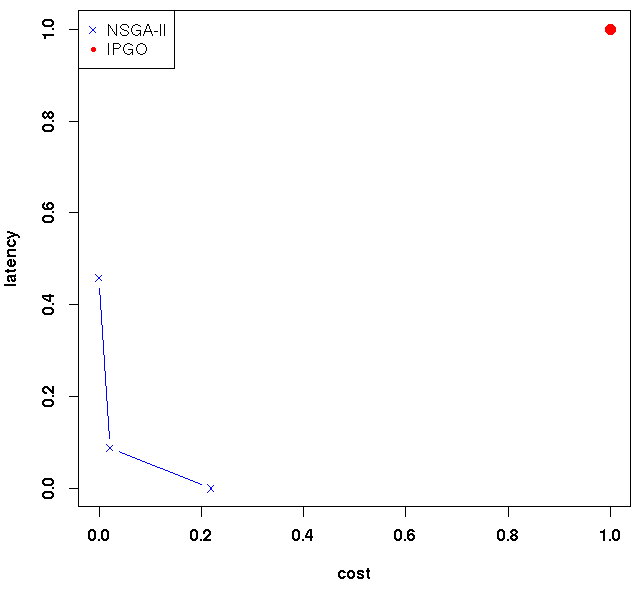
\includegraphics[width=\textwidth]{pics/122.png}
		\caption{$3 \times 3$}
		\label{fig:3_3}
	\end{subfigure}%
	\begin{subfigure}[b]{0.49\textwidth}
		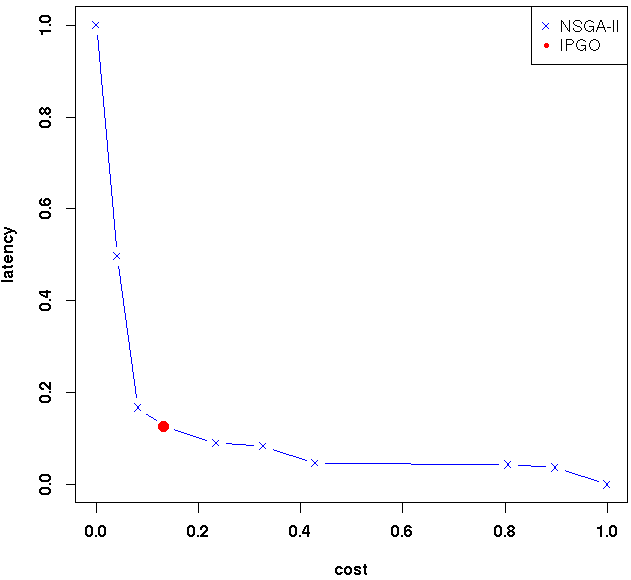
\includegraphics[width=\textwidth]{pics/123.png}
		\caption{$5 \times 5$}
		\label{fig:5_5}
	\end{subfigure}


	\begin{subfigure}[b]{0.49\textwidth}
		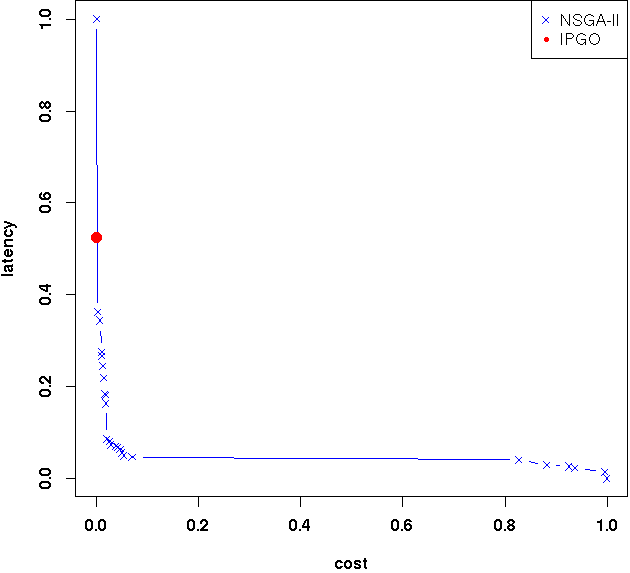
\includegraphics[width=\textwidth]{pics/124.png}
		\caption{$10 \times 10$}
		\label{fig:10_10}
	\end{subfigure}
	\begin{subfigure}[b]{0.49\textwidth}
		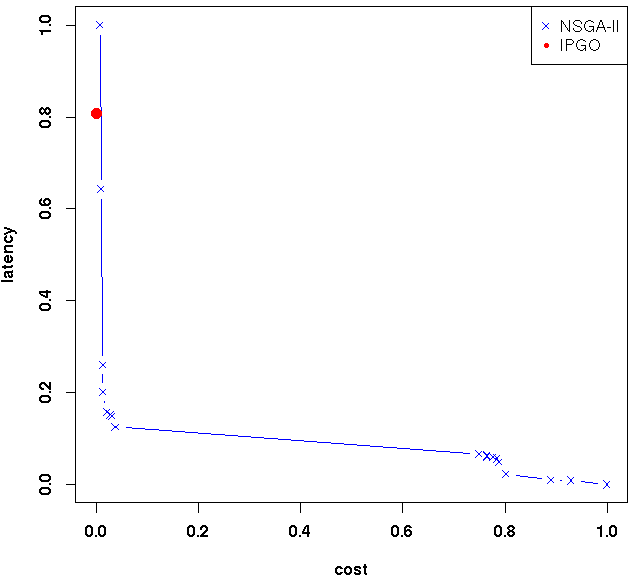
\includegraphics[width=\textwidth]{pics/125.png}
		\caption{$15 \times 15$}
		\label{fig:15_15}
	\end{subfigure}

	\caption{}\label{fig:condition}
\end{figure}
We conducted 16 experiments on 4 datasets under 4 cost constraints: sufficient, good, poor and minimum. The results show similar 
patterns for same dataset. Therefore, we only show one figure for each dataset.


Figure \ref{fig:3_3} shows NSGA-II is outperforms IPGO. As we discussed in the previous section, the 
result of IPGO is dominated by NSGA-II's solution set. \ref{fig:5_5} \ref{fig:10_10} \ref{fig:15_15} show that solution of IPGO is on the Pareto front. It does not improve the quality of the solution
set. Therefore, we considered NSGA-II outperforms IPGO in this case. The solution from IPGO is non-dominated solution in the NSGA-II solution set. While the inclusion
of the IPGO solution somewhat improves the quality of the NSGA-II solution set, we cannot say that IPGO outperforms NSGA-II since the 
IPGO solution dominates no NSGA-II solutions.

As a whole, NSGA-II can provide a set of solutions which allow user to choose according to their preference. Further, the set of 
solutions always contains the best solutions resulted from IPGO, which shows stronger problem solving ability than IPGO.


\section{Conclusion}
In this paper, we proposed a NSGA-II based approach to web service location-allocation problem. 
Our approach utilizes a memory pool so that
greatly reduces the evaluation time while the diversity of the population gradually decreases. We have conducted a full experimental evaluation using the public WS-DREAM dataset to compare our approach to Alternate Location Allocation algorithm. 
The experimental results shows the NSGA-II is effective to provide a near-optima solutions for the web service location-allocation problem.

\bibliography{llncs}
\bibliographystyle{splncs03}

% that's all folks
\end{document}
